\documentclass[UTF8]{book}
\usepackage{ctex}
\usepackage{amsmath}
\usepackage{txfonts}
\usepackage{amssymb}
\usepackage{times}
\usepackage{graphicx}
\usepackage{epsfig,tabularx,amssymb,amsmath,subfigure,multirow}
%\usepackage{algorithmic}
\usepackage[linesnumbered,ruled,noend]{algorithm2e}
\usepackage[noend]{algorithmic}
\usepackage{multirow}
\usepackage{graphicx,floatrow}
\usepackage{listings}
\usepackage{threeparttable}
\usepackage[T1]{fontenc}
\usepackage{pgfplots}
\usepackage{tikz}
\usepackage{filecontents}
\usepackage[style=numeric,backend=bibtex]{biblatex}

\newcommand{\nop}[1]{}
\newcommand{\tabincell}[2]{\begin{tabular}{@{}#1@{}}#2\end{tabular}}
\newtheorem{definition}{定义}[chapter]
\newtheorem{proposition}[definition]{\hei 命题}
\newtheorem{assumption}[definition]{\hei 假设}
\newtheorem{lemma}[definition]{\hei 引理}
\newtheorem{remark}[definition]{\hei 注}
%\newtheorem{theorem}{\hei 定理}[chapter]
\newtheorem{theorem}[definition]{\hei 定理}
\newtheorem{axiom}{\hei 公理}
%\newtheorem{algorithm1}[definition]{\hei 算法}
\newtheorem{corollary}[definition]{\hei 推论}

\newtheorem{proof}{\hei 证明}

\newtheorem{example}{例}[chapter]

\addbibresource{reference.bib}


\begin{document}

\title{\huge 知识图谱原理及应用}

\author{彭鹏,邹磊,洪亮}

\date{\today}

\maketitle

\newpage

\tableofcontents

\newpage

\part{基础知识}
\chapter{知识图谱概述}\label{sec:Background}
\section{什么是知识图谱}
当我们在百度“瓦特”的时候,百度会返回发明家瓦特的百度百科等页面(如图\ref{fig:baiduWatt})。为什么会这样?
因为百度为所有网页建立了从关键词到网页的倒排索引。基于倒排索引,百度首先找到了包含“瓦特”的网页,然后百度基于PageRank算法对这些网页按照权威程度进行排序,最后最权威的网页(如瓦特的百度百科页面)被排在前面返回给我们。

换言之,瓦特的百度百科页面被返回的原因并不在于计算机知道那个网页描述了瓦特,而是在于这个网页包含了“瓦特”这两个字。

\begin{figure}
\begin{center}
   \includegraphics[width=12cm]{./figures/part1/baidu.png}
    \caption{百度“瓦特”结果页面}
   \label{fig:baiduWatt}
\end{center}
\end{figure}


上面这些基于文本字符串的技术,在这些年的互联网发展中取得不错的效果,已经成为了目前互联网上进行自然语言理解的基础。谷歌、百度等一系列搜索引擎基于这些技术成长为了行业巨头。


但是随着时代发展,这些技术的局限性也日益明显。因为基于文本字符串的技术本质上并没有理解我们的语义,所以它无法处理复杂的带语义的查询。比如当我们查询“瓦特在哪工作过?”的时候,百度会给我们返回一系列百度知道、百度贴吧的问答(如图\ref{fig:baidufatherinlaw}),而无法直接返回“格拉斯哥大学”的相关页面。这本质上就是因为搜索引擎只是根据网页中的文本内容来得到结果,而不是真正理解我们的世界。

\begin{example}\textbf{(背景知识)}

\emph{詹姆斯·瓦特}(James Watt,1736年1月19日 — 1819年8月25日)英国发明家,出生于苏格兰的港口小镇格林诺克(Greenock),第一次工业革命的重要人物。他于1776年制造出第一台有实用价值的蒸汽机,进而开辟了人类利用能源新时代,使人类进入“蒸汽时代”。后人为了纪念这位伟大的发明家,把功率的单位定为“瓦特”(简称“瓦”,符号W)。\footnote{https://baike.baidu.com/item/詹姆斯·瓦特}

\emph{格拉斯哥大学}(University of Glasgow),英国老牌名校,位于英国苏格兰格拉斯哥市,始建于1451年,是全球最为古老的十所大学之一,英语世界国家第四古老大学。
作为一所英国综合性古典大学,格拉斯哥大学与人类文明的发展紧密相联。经济学之父亚当·斯密(Adam Smith)、工业革命之父詹姆斯·瓦特等大批杰出校友均为社会的发展进步做出了举世瞩目的贡献。\footnote{https://baike.baidu.com/item/格拉斯哥大学}

1757年,格拉斯哥大学的教授提供给瓦特一个机会,让他在大学里开设了一间小修理店。其中的一位教授,物理学家与化学家约瑟夫·布莱克(Joseph Black)更是成了瓦特的朋友与导师。瓦特的小店开业5年后,在朋友的引导下,瓦特开始了对蒸汽机的实验。经过近20年的研发,1774年瓦特将自己设计的蒸汽机投入生产,并于1776年成功制造了第一批新型蒸汽机并应用于实际生产。
\end{example}

\begin{figure}
\begin{center}
   \includegraphics[width=12cm]{./figures/part1/baidufatherinlaw.png}
    \caption{百度“瓦特在哪工作过?”结果页面}
   \label{fig:baidufatherinlaw}
\end{center}
\end{figure}

为了让计算机更加智能,让计算机理解我们的世界,于是我们需要计算机理解这个世界的知识。


知识是结构化的经验、价值、相关信息和专家洞察力的融合,并为新经验的评估、整合与资讯等提供架构\cite{url:KnowledgeDef}。20世纪90 年代以来,万维网已成为人们获取知识的主要的手段\cite{article:Internet}。为了在万维网上的获取知识,人们通常通过向搜索引擎提交关键词的方式从万维网上检索出通过网页文本、图片、视频等形式所呈现出的信息,并从这些信息里面提取所需知识。


近些年来,知识图谱(Knowledge Graph)逐渐兴起并成为互联网上表示知识并利用知识的重要发展方向。知识图谱是由谷歌公司于2012年5月16日正式发布出来,用来增强谷歌搜索引擎的能力\cite{url:KnowledgeGraphDef}。
在知识图谱中,人们将越来越多的知识按照图的形式结构化地组织起来。这些图结构化、易操作、易利用、全面有组织的知识集群就是知识图谱。知识图谱经常是采用某种知识表示模型在计算机存储器中存储、组织、管理和使用的互相联系的知识片集合。

构建知识图谱的本质,就是让机器具备认知能力,理解这个世界。

\section{知识图谱由来与发展}
知识图谱源于专家系统与知识工程,是人工智能学科符号主义分支的最新研究成果。
1956年夏,麦卡锡、明斯基等科学家在美国达特茅斯学院开会研讨“如何用机器模拟人的智能”,首次提出“人工智能(Artificial Intelligence,简称AI)”这一概念,标志着人工智能学科的诞生。而这些科学家都是符号主义者。正是这些符号主义者,早在1956年首先采用“人工智能”这个术语。直到2012年,谷歌提出了“知识图谱”概念,将符号主义这一分支又推向了新的高度。

知识图谱这个概念虽然是2012年之后才为大家所知的,但是这个技术继承了符号主义几十年的积累。从1956年人工智能学科符号主义分支形成以来,符号主义分支走过了一条启发式算法——专家系统——知识工程的发展道路。

在六十年代、七十年代的时候,知识工程这个领域往前发展,不断的产生出新的逻辑语言和新的实用方法,像描述逻辑是七十年代就兴起了的。在六十年代时就有一个叫语义网络。注意,不是“语义网”而是“语义网络 ”,那个时候的语义网络跟现在的知识图谱非常像。所以这个是不断循环的,如果我们把六十年的学科发展抽象来看,实际上就是一个从简单到复杂、再从复杂回归简单的过程。

从最终得到的结果来看,好像我们现在得到的知识图谱跟六十年代就已经有的语义网络非常像,但这种像只是表面上的。因为在发展过程中,我们构造了一个庞大的工业体系,以及如何从各种各样的文档、各种各样的数据里集中编辑、生成知识图谱的一整套工业链。所以一个技术不能只看它的定义,而是要看它相关所有实践过程中工业体系的总和。今天知识图谱的技术无论从深度还是广度上,都远远超越六十年代的语义网络技术。

八十年代、九十年代、到两千年,这中间还有非常多中间技术,我们从中选些重要的事情说一下。

这张图是对前面那张图的抽象,我们选其中发展过程中最重要的节点。六十年代有一种东西叫 “ 语义网络 ”,语义网络在七十年代、八十年代时演化成了描述逻辑。为什么会有这种变化?因为语义网络本身只是一种表征,并不具备推理能力。语义网络 + 推理变成了新的逻辑系统,叫 “ 描述逻辑 ”,描述逻辑到两千年前后跟 Web 技术结合在一起,形成了新的语言,比如 OIL 、DAML。

另外一个分支是 1995 年前后有了元数据,从元数据学科衍生出一个分支叫 RDF,后来 RDF 和 DAML 合并起来就变成了 OWL。下面还有一些更工程的内容,包括 schema.org、RDFa、JOSN-LD、GraphpDB,这都是最近 5、6 年兴起的新技术。这些技术的总和就构成了我们所称的 “ 知识图谱 ” 技术,但只是其中一部分。

给大家看一个语义网络,语义网络其实就是一个网络。这张图上有各种不同的概念,比如中间的 Mammal 是哺乳动物,猫(cat) 是一种哺乳动物,猫有毛;熊是哺乳动物,熊也有毛;鲸是一种哺乳动物,鲸在水里面生活;鱼也在水里面生活,也是一种动物;哺乳动物是一种脊椎动物,也是动物的一种。

所有这些节点和边的总和就构成了一个网络,每一条边上都有一些标志的,用术语来说就是 “ 有类型的边 ”,这种 “ 有类型的边 ” 连在一起的节点叫 “ 语义网络 ”,概念是非常简单的。

六十年代时自然语言处理和知识表现的大拿批评这种语义网络,说这个东西没办法用于推理,用术语来说是最后没有 “ semantics ”。

这里涉及很多关系,什么叫 semantics?有的学者认为 semantics 必须是有一套严格的语义定义,这通常是用模型论来定义,或者过程方法来定义。其实也有更浅的对语义的理解,万事万物之间的关系就是语义。比如我们打开字典,字典是用一些词定义另外一些词,这就是语义。

我们在这样的语义网络里,如何定义一个词的意义?其实我们是做不到的。比如在这个语义网络里,居于中间位置的词是“哺乳动物”,它到底是什么?我们很难让计算机理解什么是真正的哺乳动物,很难通过它的内涵含义来理解。对于计算机而言,它只能知道万事万物之间的联系,也许这对于机器自动处理来说就够了。所以语义网络尽管没有所谓的语义,我们还是把它称为语义网络的原因,因为语义就是关系。


到了八十年代时,描述逻辑就已经比较成熟了。描述逻辑是逻辑的一种,我在这里面列了一张表,这是描述逻辑和一阶逻辑 (FOL 逻辑)之间的对应。如果大家没有逻辑基础也不用害怕,因为这个图本质上是讲很基础的逻辑定义。

我们有了一个描述逻辑之后,就可以用计算机来做一些自动推理的工作。八十年代到九十年代,描述逻辑学者们一直都在寻找如何让计算机更好的进行逻辑推理,一些比较可判定的所谓计算机不会死机的那些问题的总和,这种语言称为 “ 描述逻辑 ”。


到九十年代时描述逻辑成为知识表现领域的一种非常显学、非常重要的分支,正好这时互联网兴起了。到了 1995 年前后开始了真正知识图谱化的第一步,开始把描述逻辑用互联网的语言来重新来表征,有人用 HTML,也有人用 XML。1999 年马里兰大学开始发布了第一个这样的语言,叫 “ SHOE ”。后来这个语言被美国的国防部高等研究所资助了一个项目叫 “ DAML ”,这就是第一个在美国这边把知识表现语言放在网上一种官方的努力。

与此同时,在欧洲也有一个非常相似的努力叫 “ OIL ”,大西洋两岸的同行们一看,大家做的事情非常相似,于是在 2001 年时 W3C 开始把两边的努力汇总在一起,出现了一个语言叫 “ DAML + OIL ”。到了 2004 年时 W3C 进一步协调大家的努力,合并了一个新的语言叫 “ OWL ”,2009 年发布了第二版,叫 “ OWL2 ”。

从九十年代到 2009 年这十几年期间,这个领域不断向上、向好积极发展,在那个时候我们曾经认为 OWL 是描述这个世界非常好的一种工具,因为它对于机器处理是非常友好的,所以我们就希望把它放到互联网上去,让更多人用到,但是这个设想后来并没有实现。


这里多说几句 OWL,因为我是 OWL 工作组的一员,所以知道一些早期的事情。OWL有两个工作组,最早的一个工作组是在 2000 - 2004 年之间,我赶上的是 2007 - 2010 年的第二个工作组,这个工作组的使命是把现有的 OWL 语言进一步完善,提供所谓更强的表达力,或者在机器处理上比如要进行语义数据的查询,我们应该用什么样的,什么可以用、什么不能用、什么能说、什么不能说、什么对机器是友好的,OWL 工作组就是做这个事情。

我们写了 10 来个文档,加在一起 600 多页纸,花了两年时间做这个事情。OWL 工作组除了大学里来的人,还有一些企业的成员,包括 IBM、Oracle、惠普等等,还有一些小的创业公司。

那个时候我们这个领域遇到了一些瓶颈的,就是 OWL 这个语言或者语义网整个领域,在 2000 年前后是大家非常寄予厚望的,就好像现在大家对于深度学习寄予厚望一样。但是往前走到 2006 年前后遇到了瓶颈,就是没有人真的去产生这样的数据,大多数日常场景用不到语义。于是这时候就产生了内部的路线斗争,叫 “ SEMANTIC Web or semantic WEB ”,就是到底我们是加强语义呢?还是加强互联网属性呢?有两组不同的人不断进行争执。

当然,还有很多其他的分歧,包括我们到底该怎么去定义什么叫 “ 简单 ”,大家没有一致的意见。所以我们最终生成的文档从学术角度来说是非常有价值,但是对于工业应用特别是 C 端的互联网应用没有达到预期。


前面这一段大体总结了知识图谱技术发展的前两个大的阶段历史,一个是从六十年代到九十年代,早期知识图谱的原型,包括语义网络等等,后面一系列的技术。

从 2001 - 2006 年或者 2007 年这段时间,是不断加强语义网所谓的语义的过程,就是从弱语义到强语义,从语义网络到描述逻辑,一直发展到 OWL,并行还有另外其他一些,比如基于框架逻辑还有另外一个语言叫 “ RIF ”。

这十几年时间都一直不断在加强语义表现的表达力,但最后证明这个做法是不太妥当的。


我们讲过,除了学术性非常强的描述逻辑 OWL 分支之外,知识图谱还有另外一个分支是来自于元数据框架的。这个工作最早是 Guha 在 Apple 做的,Guha 这个人是非常值得关注的,因为某种程度上他是 “ 知识图谱之父 ”,在 1995 年时他在 Apple 发明了一个语言叫 “ MCF ”,因为他那时候面临一些问题,就是怎么去表征多媒体的数据,特别是图像的数据,所以他就发明了一整套的元数据表征方法。

到了 1997 年时 Guha 跟Tim Bray 做了 RDF / XML。1999 年网景公司发明了 RSS 语言,这个东西现在新一代的朋友们不一定知道了,回到 10 年前时看新闻都是用 RSS 订阅的,其实 RSS 的第一个 R 就是 RDF。后来他们改了其他的名字,从本源上来讲,技术刚刚开始的时候这个技术是 RDF 的应用。1999 年 RDF 被 W3C 收编了,变成了国际标准。


RDF 和一开始提到描述逻辑方法是不一样的,因为描述逻辑方法是从实验室里来的,它想构造一个庞大的体系,构建一个完美的知识表现语言,然后再寻找它的落地。

而 RDF 从一开始就是一个从实践出发的、自底向上的一个语言。RDF 相对于 OWL 而言,是一个更加偏工程的、应用更多的语言,现在有很多人在用 RDF。我们日常生活中所遇到的绝大多数网站,现在都有某种类型的元数据,其中相当一部分就是用 RDF 不同的变种来实现的,所以 RDF 总的来说是一个比较成功的技术,因为它是来自于现实的技术。

从 2001 年这个领域正式形成,到 2006 年时语义网的技术堆栈已经变得非常复杂了。1999 年时有一个所谓的 “ 语义网蛋糕模型 ”,对语义网不同的技术做了罗列。2006 年时语义网技术已经复杂到没有人看得懂,没有办法用二维表达,必须用一个三维的图才能够把语义网所有的技术放在里面。这就带来了一个严重的问题,就是绝大多数的企业、开发者很难理解,无从下手。


当前,人类社会业已积累大量知识。特别是,近几年在知识图谱技术的推动下,对于机器友好的各类在线知识图谱大量涌现。知识图谱本质上是一种语义网络,表达了各类实体、概念及其之间的语义关系。相对于传统知识表示形式(诸如本体、传统语义网络),知识图谱具有实体/概念覆盖率高、语义关系多样、结构友好(通常表示为RDF格式)以及质量较高等优势,从而使得知识图谱日益成为大数据时代和人工智能时代最为主要的知识表示方式。能否利用蕴含于知识图谱中的知识指导深度神经网络模型的学习从而提升模型的性能,成为了深度学习模型研究的重要问题之一。

知识图谱是人工智能符号主义近期进展的典型代表。知识图谱中的实体、概念以及关系均采用了离散的、显式的符号化表示。而这些离散的符号化表示难以直接应用于基于连续数值表示的神经网络。为了让神经网络有效利用知识图谱中的符号化知识,研究人员提出了大量的知识图谱的表示学习方法。知识图谱的表示学习旨在习得知识图谱的组成元素(节点与边)的实值向量化表示。这些连续的向量化表示可以作为神经网络的输入,从而使得神经网络模型能够充分利用知识图谱中大量存在的先验知识。这一趋势催生了对于知识图谱的表示学习的大量研究。本章首先简要回顾知识图谱的表示学习,再进一步介绍这些向量表示如何应用到基于深度学习模型的各类实际任务中,特别是问答与推荐等实际应用。


\begin{example}\textbf{(人工智能的主流学派:符号主义和联结主义)}


\emph{符号主义}是一种基于逻辑推理的智能模拟方法,其原理主要为物理符号系统(即符号操作系统)假设和有限合理性原理,长期以来,一直在人工智能中处于主导地位。该学派认为:人类认知和思维的基本单元是符号,而认知过程就是在符号表示上的一种运算。它认为人和计算机都是一个物理符号系统,所以我们就能够用计算机来模拟人的智能行为,即用计算机的符号操作来模拟人的认知过程。可以把符号主义的思想简单的归结为“认知即计算”。符号主义的代表成果是1957年纽威尔和西蒙等人研制的成为“逻辑理论家”的数学定理证明程序LT。之后,符号主义走过了一条启发式算法——专家系统——知识工程的发展道路。2012年谷歌公司发布“知识图谱”的概念,将符号主义推向了新的高潮。\footnote{https://baike.baidu.com/item/符号主义}


\emph{联结主义}
认为人工智能源于仿生学,特别是对人脑模型的研究。它的代表性成果是1943年由生理学家麦卡洛克和数理逻辑学家皮茨创立的脑模型,即MP模型。它从神经元开始进而研究神经网络模型和脑模型,开辟了人工智能的又一发展道路。20世纪60-70年代,联结主义,尤其是对以感知机为代表的脑模型的研究出现过热潮。1982年和1984年,霍普菲尔德教授发表两篇论文提出用硬件模拟神经网络。1986年,鲁梅尔哈特等人提出多层网络中的反向传播算法算法。2016年由谷歌公司的团队基于神经网络开发的阿尔法围棋与围棋世界冠军、职业九段棋手李世石进行围棋人机大战,以4比1的总比分获胜。这一消息再度极大地激发人工神经网络的研究热情,使之成为了目前最火热的人工智能流派。\cite{book:AI}


\end{example}


\section{知识图谱的数据模型与查询语言}
现阶段,人们已提出过各种各样的知识表示模型,其中以W3C提出的RDF\cite{url:RDF}最为有名且已经被广泛地应用在各个领域。在定义RDF数据模型的同时,W3C也定义了结构化查询语言SPARQL(Simple Protocol and RDF Query Language)\cite{url:sparql},以实现针对大规模RDF数据的查询与管理。目前,SPARQL查询语言已经成为W3C 的RDF 查询语言的推荐标准。本章将简述RDF和SPARQL的定义,并在第\ref{sec:RDFIntroduction}章和第\ref{sec:SPARQLIntroduction}章,我们将详细分别介绍RDF和 SPARQL的定义。




RDF (Resource Description Framework,即资源描述框架) 是W3C提出的一组知识表示的模型,以便更为丰富地描述和表达网络资源的内容与结构。RDF利用统一资源标识符(Uniform Resource Identifier,URI)标识从网页等信息资源拓展到所有事物。这些URI 所对应的事物既包括真实世界中的实体(比如一本书)也包括人们在社会实践中形成的概念(比如书、作者)等。这些URI 所对应的事物又被成为资源。这些资源很多都是有自己的属性描述的;此外,客观世界中不同实体、概念和事件相互之间可能会有各种关系,所以知识图谱数据中不同资源之间也是会有关系的。


例如,图\ref{fig:rdfresource}以DBpedia\cite{DBLP:DBpedia}中瓦特为例来表示了知识图谱中对资源的描述。瓦特人像上方的字符串标识符就是瓦特所对应资源的URI。图\ref{fig:rdfresource}中瓦特人像下方给出的属性和属性值描述了瓦特这个资源所对应的人的名字是“James Watt”@en。图\ref{fig:rdfresource}给出了瓦特和另一个表示格拉斯哥大学所对应的资源通过一个“dbp:workplaces”关系连接了起来,描述了瓦特与格拉斯哥大学有“工作地点”这个关系,即瓦特在格拉斯哥大学工作。

\begin{figure}[h]
\begin{center}
   \includegraphics[width=9cm]{./figures/part1/resource.pdf}
    \caption{RDF资源}
   \label{fig:rdfresource}
\end{center}
\end{figure}

RDF的基本数据单元是一个三元组,可以表示为<主体,属性,客体>。每个三元组表示某个资源的一个属性值或者某个资源与其他资源的关系。当某条三元组描述了某个实体的属性时,其三个元素也被称为主体、属性及属性值。因此,一个知识图谱数据集可以看做一系列三元组的集合。

例如,图\ref{fig:rdftriples}中展示了一个RDF数据集的片段。这段数据截取于著名的RDF数据集DBPedia\cite{DBLP:DBpedia},描述了工业革命时期与瓦特相关的人物以及相关事物所对应的资源以及它们之间的关系。

\begin{figure}
\begin{center}
   \includegraphics[width=12cm]{./figures/part1/triples.pdf}
    \caption{RDF三元组示例}
   \label{fig:rdftriples}
\end{center}
\end{figure}

%\subsection{RDF数据图模型}\label{sec:RDFGraphModel}
利用这些属性和关系,很多实体就被连接起来形成了一个大的知识图谱。按照上述的描述,我们可以发现一个知识图谱数据可以天然的被视为一个图。在这个图中,每个实体或者知识图谱数据集中出现过的字符串可以被视为图上的点,每个三元组可以视为连接主体及客体的有向边,而三元组中的谓词就可以视为有向边上的标签。相比于将知识图谱数据视为XML格式数据或三元组的集合,知识图谱的图模型包含了知识图谱数据中涵盖的语义信息。


图\ref{fig:datagraph}就是图\ref{fig:rdftriples}所示知识图谱三元组数据的图形式。如图\ref{fig:datagraph}所示,知识图谱可以表示成一个有向图,其所有的实体都是椭圆,概念是圆形,而文本点都是矩形点。


\begin{figure}
\begin{center}
   \includegraphics[width=12cm]{./figures/part1/data_graph.pdf}
    \caption{RDF数据图}
   \label{fig:datagraph}
\end{center}
\end{figure}

另一方面,SPARQL 语言与目前关系数据库中的SQL 语言是很相近的。在SPARQL 语法中,也是用SELECT 语句查询满足特定条件的RDF数据片段。具体而言,对于一个SELECT 语句中,SELECT 子句指定查询应当返回的内容,FROM 子句是指定将要使用的数据集,WHERE 子句一组三元模式组成用以指定所返回的RDF 数据片段需要满足的模式。SPARQL 语言与SQL 语言相似的这个特性方便了用户对于SPARQL 语言的使用。图\ref{fig:SPARQLStatements}(a)给出了一个针对哲学家的简单的 SPARQL 查询,目标在于查询出``在格拉斯哥大学工作的人都受到哪些人的影响?''。

\nop{
\small{
\begin{lstlisting}[language=SQL]
SELECT  ?x ?n  WHERE
{?x mainInterest Ethics.
?x influencedBy Aristotle.
?x name ?n. }
\end{lstlisting}
}
\normalsize
}

与RDF数据的图形式表示类似,一个SPARQL 查询可以表示为一个查询图\cite{VLDB2011:gStore,VLDBJ:gStore},查询中每个变量或者常量对应一个查询图上的点,每个WHERE 子句中的三元模式对应一条边。例如,图\ref{fig:SPARQLStatements}(b) 就给出了图\ref{fig:SPARQLStatements}(a)中示例SPARQL 所对应的查询图。


\begin{figure}[h]
\begin{center}
   \includegraphics[width=11cm]{./figures/part1/query_graph.pdf}
    \caption{SPARQL查询图示例}
   \label{fig:SPARQLStatements}
\end{center}
\end{figure}

\section{知识图谱的价值}
知识图谱用节点和关系所组成的图谱,为真实世界的各个场景直观地建模,运用“图”这种基础性、通用性的“语言”,“高保真”地表达这个多姿多彩世界的各种关系,并且非常直观、自然、直接和高效,不需要中间过程的转换和处理——这种中间过程的转换和处理,往往把问题复杂化,或者遗漏掉很多有价值的信息。

在风控领域中,知识图谱产品为精准揭露“欺诈环”、“窝案”、“中介造假”、“洗钱”和其他复杂的欺诈手法,提供了新的方法和工具。尽管没有完美的反欺诈措施,但通过超越单个数据点并让多个节点进行联系,仍能发现一些隐藏信息,找到欺诈者的漏洞,通常这些看似正常不过的联系(关系),常常被我们忽视,但又是最有价值的反欺诈线索和风险突破口。

尽管各个风险场景的业务风险不同,其欺诈方式也不同,但都有一个非常重要的共同点——欺诈依赖于信息不对称和间接层,且它们可以通过知识图谱的关联分析被揭示出来,高级欺诈也难以“隐身”。

凡是有关系的地方都可以用到知识图谱,事实上,知识图谱已经成功俘获了大量客户,且客户数量和应用领域还在不断增长中,包括沃尔玛、领英、阿迪达斯、惠普、FT金融时报等知名企业和机构。

目前知识图谱产品的客户行业,分类主要集中在:社交网络、人力资源与招聘、金融、保险、零售、广告、物流、通信、IT、制造业、传媒、医疗、电子商务和物流等领域。在风控领域中,知识图谱类产品主要应用于反欺诈、反洗钱、互联网授信、保险欺诈、银行欺诈、电商欺诈、项目审计作假、企业关系分析、罪犯追踪等场景中。

那相比传统数据存储和计算方式,知识图谱的优势显现在哪里呢?

\begin{itemize}
  \item \textbf{关系的表达能力强.}传统数据库通常通过表格、字段等方式进行读取,而关系的层级及表达方式多种多样,且基于图论和概率图模型,可以处理复杂多样的关联分析,满足企业各种角色关系的分析和管理需要。
  \item \textbf{像人类思考一样去做分析.}基于知识图谱的交互探索式分析,可以模拟人的思考过程去发现、求证、推理,业务人员自己就可以完成全部过程,不需要专业人员的协助。
  \item \textbf{知识学习.}利用交互式机器学习技术,支持根据推理、纠错、标注等交互动作的学习功能,不断沉淀知识逻辑和模型,提高系统智能性,将知识沉淀在企业内部,降低对经验的依赖。
  \item \textbf{高速反馈.}图式的数据存储方式,相比传统存储方式,数据调取速度更快,图库可计算超过百万潜在的实体的属性分布,可实现秒级返回结果,真正实现人机互动的实时响应,让用户可以做到即时决策。
\end{itemize}



\section{知识图谱的应用}
知识图谱的应用场景很多,在不同行业不同领域也有广泛应用。在本书中,我们将以几个目前比较常见的应用场景为例像大家介绍一下知识图谱应用。

\subsection{基于金融知识图谱的股权分析}

\subsection{基于医疗知识图谱的辅助诊断}


\subsection{基于知识图谱的智能问答}
\chapter{知识图谱管理所使用的背景知识}
\section{图论}
过去几十年间,人们对现代社会发展中形成的``连通性''产生了日益浓厚的兴趣。这种兴趣的核心就是\emph{图}(graph)。图是事物之间相互关系的一种模式,人们在很多场合的讨论和报道中都会提到。实际应用中,已经出现了各式各样的图,如社交网络、知识图谱等等。这些图规模巨大,结构复杂,包含丰富的信息,为帮助人们更好地生产生活提供了丰富的信息源。


为此,本章将主要从图论的角度来作为知识图谱的基础知识。

\subsection{图的基本定义}
图论作为网络的基础最早是由瑞士著名数学家欧拉针对哥尼斯堡七桥问题所提出的。如今,图论已经成为了离散数学的一个重要分支,被广泛地在应用在各个领域。


\begin{example}
\textbf{哥尼斯堡七桥问题}
哥尼斯堡七桥问题是18世纪著名古典数学问题之一,欧拉通过求解这个问题奠定了图论。在哥尼斯堡的一个公园里,有七座桥将普雷格尔河中两个岛及岛与河岸连接起来(如图\ref{fig:graph:KnigsbergBridge}中左图所示)。问是否可能从这四块陆地中任一块出发,恰好通过每座桥一次,再回到起点?

\begin{figure}[htbp]
	\centering\includegraphics[width=3.5in]{./figures/part1/KnigsbergBridge.jpg}
	\caption{哥尼斯堡七桥问题示例图}\label{fig:graph:KnigsbergBridge}
\end{figure}

欧拉于1736年研究并解决了此问题,他把问题归结为如图\ref{fig:graph:KnigsbergBridge}中右图所示图上的``一笔画''问题。欧拉不仅解决了此问题,且给出了连通图可以一笔画的充要条件是:有奇数个相邻边的点不是没有就是两个。证明思路在于要想一笔画成,中间路过点必须均是偶数条相邻变,也就是有来路必有另一条去路,有奇数个相邻边的点要么没有要么在两端。
\end{example}



%\subsection{基本定义}\label{sec:graphdefinition}
这里所说的\emph{图},是以一种抽象的形式来表示若干对象结合以及这些对象之间的关系。


\begin{definition}
\label{def:graph}
\textbf{图}:图表示成一个二元组$G=(V,E)$,其中V 是点集合;E 表示边集合,其中每条边由V中两个点相连接所构成。构成一条边的两个点称之为这条边的端点。一条边的两个端点可以是V中的相同或者不同点,两个端点相同的边称之为\emph{环}。
\end{definition}

如果E中的边都是没有方向的,那么G被称为无向图;如果E中的边是有方向的,那么G被称为有向图。
给定V中的两个元素u和v,如果它们之间存在一条无向边,则记为$e=(u,v)\in E$;如果它们之间存在一条有向边,则记为$e=\langle u,v\rangle \in E$,其中u被称为起点,v被称为终点。
此外,G中的边$e$可以被赋上一个权重,记为$w(e)$。

\begin{definition}
\label{def:graph_degree}
\textbf{度数}:给定一个无向图$G=(V,E)$,对于任意的$v\in V$,称v作为G中边的端点的次数之和为v的\emph{度数},简称\emph{度},记作$deg_G(v)$,在不发生混淆的情况下,也可以简写为$deg(v)$。

给定一个有向图$G=(V,E)$,对于任意的$v\in V$,称v作为G中边的起点的次数之和为v的\emph{出度},记作$deg_G^+(v)$,简记作$deg^+(v)$;称v作为G中边的终点的次数之和为v的\emph{入度},记作$deg_G^-(v)$,简记作$deg^-(v)$。$deg^+(v)+deg^-(v)$被称为v的度数,记作$deg(v)$。
\end{definition}

\begin{example}
图\ref{fig:graph:ExampleGraph}给出了一个无向图和有向图的示例。其中,对于图\ref{fig:graph:ExampleGraphUndirected}中点3而言,它的度数是4;对于图\ref{fig:graph:ExampleGraphDirected}中点3而言,它的入度是3,出度是1,度数是4。

\begin{figure}[h]
   \centering
\subfigure[][{无向图}]{%
      \includegraphics[scale=0.75]{./figures/part1/undirected_graph.pdf}
       \label{fig:graph:ExampleGraphUndirected}%
       }
       \hspace{0.1in}
   \subfigure[][{有向图}]{%
      \includegraphics[scale=0.75]{./figures/part1/directed_graph.pdf}
       \label{fig:graph:ExampleGraphDirected}%
       }%
 \caption{ 图示例}%
\vspace{-0.2in}
 \label{fig:graph:ExampleGraph}
\end{figure}
\end{example}

图的表示方式有很多种。不同的表示方式适用于不同的应用。其中最常见的两种表示方式就是:\emph{邻接表}和\emph{邻接矩阵}。

给定图$G=(V,E)$,它的邻接表就是给出图中每个点相邻的相邻的点。
给定无权图$G=(V,E)$,其中$|V|=n$,且V中的点编号为$v_{1},v_2,...,v_{n}$,G的邻接矩阵$\mathbb{A}=[a_{i,j}]$是一个$n\times n$的0-1矩阵,它满足这样的性质:若存在一条边$e=(v_i,v_j)\in E$,则$a_{i,j}=1$;否则,$a_{i,j}=0$。若是有权图,若存在一条边$e=(v_i,v_j)\in E$,则$a_{i,j}=w(e)$。图\ref{fig:graph:ExampleGraphRepresentation}给出了图\ref{fig:graph:ExampleGraphUndirected}所示图的邻接表和邻接矩阵。

\begin{figure}[h]
   \centering
\subfigure[][{邻接表}]{%
      \includegraphics[scale=0.8]{./figures/part1/adjacent_list.pdf}
       \label{fig:graph:ExampleAdjacentList}%
       }
       \hspace{0.05in}
   \subfigure[][{邻接矩阵}]{%
      \includegraphics[scale=0.65]{./figures/part1/adjacent_matrix.pdf}
       \label{fig:graph:ExampleAdjacentMatrix}%
       }%
 \caption{ 图的表示方式示例}%
\vspace{-0.2in}
 \label{fig:graph:ExampleGraphRepresentation}
\end{figure}


此外,许多问题是利用沿图中的边前进所形成的的路径来建模的。例如,判定能否从一个公路网络中的某个点行进到另一个点,就可以用图中的路径概念来建模。
定义\ref{def:graph_path}给出了路径的形式化定义和相关术语。
\begin{definition}
\label{def:graph_path}
\textbf{路径}:给定一个无向图$G=(V,E)$,G中顶点与边的交替序列$\Gamma = v_{i_0}e_{j_1}v_{i_1}e_{j_2}...e_{j_l}v_{i_l}$称为点$v_{i_0}$到点$v_{i_l}$的\emph{路径},其中$v_{i_{r-1}}$和$v_{i_{r}}$是$e_{i_r}$的端点($1\le r\le l$)。点$v_{i_0}$和点$v_{i_l}$分别被称为$\Gamma$的起点和终点。若$v_{i_0}$和点$v_{i_l}$是同一个点,则$\Gamma$被称为一条\emph{回路}。
如果$G$中任意两个顶点之间都存在一条路径,则称该图为连通图,否则,称该图为非连通图。非连通图的极大连通子图称为它的连通分量。

若图G是无权图,$\Gamma$中的边数$l$被称为$\Gamma$ 的\emph{长度};若G是有权图,那么$\Gamma$中各条边权重之和$\sum_{k=1}^{k=l} w(e_{j_k})$就是$\Gamma$的\emph{长度}。所有$v_{i_0}$和点$v_{i_l}$之间的路径中最短的那条路径称为\emph{最短路径},最短路径的长度被称为$v_{i_0}$到点$v_{i_l}$的\emph{距离},记为$d(v_{i_0},v_{i_l})$。

有向图中的路径、长度和回路的定义与无向图中定义类似,只是要注意在有向图中路径和回路中边的方向的一致性,即在$\Gamma = v_{i_0}e_{j_1}v_{i_1}e_{j_2}...e_{j_l}v_{i_l}$中,$v_{i_{r-1}}$必须是$e_{i_r}$的起点且$v_{i_{r}}$是$e_{i_r}$的终点($1\le r\le l$)。此外,若对于有向图G中任意两个不同的顶点$v_i$和$v_j$,都存在从$v_i$到$v_j$以及从$v_j$到$v_i$的路径,则称G是强连通图。有向图的极大强连通子图称为它的强连通分量。
\end{definition}

\subsection{图遍历问题}
图遍历又称图的遍历,指的是从图中的任一顶点出发,对图中的所有顶点访问一次且只访问一次。图的遍历是图的一种基本操作,图的许多其它操作都是建立在遍历操作的基础之上。



由于图本身的复杂性,所以图的遍历操作也较复杂,主要表现在以下几个方面:


\begin{itemize}
  \item 在图中,没有一个“自然”的首结点,图中任意一个顶点都可作为第一个被访问的结点;
  \item 在有向图中,从一个顶点出发,只能够访问它所在的连通分量上的所有顶点,所以为了访问所有点还需考虑如何选取下一个出发点。在无向图中,从一个顶点出发,能够访问它所在的连通分量上的所有顶点,所以为了访问所有点还需考虑如何选取其他连通分量的下一个出发点。
  \item 在图结构中,如果有回路存在,那么一个顶点被访问之后,有可能沿回路又回到该顶点;
\end{itemize}

在图中,一个顶点可以和其它多个顶点相连,当这样的顶点访问过后,存在如何选取下一个要访问的顶点的问题。根据不同选取策略,图遍历算法可以分为:深度优先遍历和广度优先遍历。

\subsubsection{宽度优先遍历}

宽度优先搜索算法(又称广度优先搜索)是最简便的图的搜索算法之一,属于一种盲目搜寻法,目的是系统地展开并检查图中的所有节点,以找寻结果。换句话说,它并不考虑结果的可能位置,彻底地搜索整张图,直到找到结果为止。


\begin{algorithm}[h] \label{alg:BFS}
\caption{宽度优先遍历}
\small
\KwIn{图$G=(V,E,L)$和遍历起点$s$}
%\KwOut{ A set ${L_{in}}\subseteq L$ for coarsening}
$level[s] \gets 0$;\\
$parent[s] \gets s$;\\
将$s$插入队列queue中;\\
\While{$queue$不为空}{
	将队列queue的首个元素$v$推出;\\
	\For{$v$的相邻点$v^\prime$}{
		\If{$v$不在level中}{
			$level[v^\prime] \gets level[v^\prime] + 1$;\\
			$parent[v^\prime] \gets v$;\\
			将$v^\prime$插入队列queue中;\\
		}
	}
}
\end{algorithm}


\subsubsection{深度优先遍历}
深度优先遍历方法在于对每一个可能的分支路径深入到不能再深入为止,而且每个节点只能访问一次。它的基本思想是:从图的某个顶点$v_0$出发,访问$v_0$,然后选择一个与$v_0$相邻且没被访问过的顶点$v_i$访问,再从$v_i$出发选择一个与$v_i$相邻且未被访问的顶点$v_j$进行访问,依次继续。如果当前被访问过的顶点的所有邻接顶点都已被访问,则退回到已被访问的顶点序列中最后一个拥有未被访问的相邻顶点的顶点$w$,从$w$出发按同样的方法向前遍历,直到图中所有顶点都被访问。


\begin{algorithm}[h] \label{alg:DFS}
\caption{深度优先遍历和遍历起点$s$}
\small
\KwIn{图$G=(V,E,L)$和遍历起点$s$}
%\KwOut{ A set ${L_{in}}\subseteq L$ for coarsening}
$level[s] \gets 0$;\\
$parent[s] \gets s$;\\
将$s$插入栈stack中;\\
\While{$stack$不为空}{
	将栈stack的栈顶元素$v$推出;\\
	\For{$v$的相邻点$v^\prime$}{
		\If{$v$不在level中}{
			$level[v^\prime] \gets level[v^\prime] + 1$;\\
			$parent[v^\prime] \gets v$;\\
			将$v^\prime$插入栈stack中;\\
		}
	}
}
\end{algorithm}



\subsection{子图匹配问题}

\section{数据库}
数据库实际上就是一个文件集合,是一个存储数据的仓库,本质就是一个文件系统,数据库是按照特定的格式把数据存储起来,用户可以对存储的数据进行增删改查操作。

数据是指描述事物的符号记录,包括数据的表现形式和数据解释两个部分。如数字、音频、图形、文本、图像、语言、视频等多种表现形式。经过数字化处理后存入计算机。

数据是信息的符号表示或载体。信息是数据的内涵是对数据的语义解释。

数据库(DB):长期存储在计算机内、有组织、可共享的大量数据的集合。数据库中的数据按照一定的数据模型组织、描述和存储,具有娇小的冗余度、交稿的数据独立性和易扩展性,并可为各种用户共享。

数据库管理系统(DBMS):位于用户和操作系统间的数据管理系统的一层数据管理软件。用途:科学地组织和存储数据,高效地获取和维护数据。包括数据定义功能,数据组织、存储和管理,数据库的事物管理和运行管理,数据库的建立和维护功能,其他功能。

数据库系统(DBS):在计算机系统中引入数据库后的系统,一般由数据库。数据库管理系统(及其开发工具)、应用系统、数据库管理员构成。目的:存储信息并支持用户检索和更新所需的信息。

关系数据结构:描述现实世界的实体以及实体间的各种联系。只包含单一的数据结构—关系。

关系操作
查询操作:选择、投影、连接、除、并、差、交、笛卡尔积等。
插入、删除、修改操作。

关系的完整性约束
实体完整性和参照完整性:关系模型必须满足的完整性约束条件称为关系的两个不变性,应该由关系系统自动支持。
用户定义的完整性:应用领域需要遵循的约束条件,体现了具体领域中的语义约束。


SQL


\chapter{知识图谱的数据模型---RDF\& OWL}\label{sec:RDFIntroduction}
\section{RDF数据三元组模型}\label{sec:RDFModel}
\indent
     从知识图谱数据组织的架构来看,可以把知识图谱的数据分为两个层次,一个是数据模型层,数据模型是按照本体论的思想,勾画出来的数据组织模式,数据模型可以展示数据的组织方式,数据之间的相互关系,创建动植物的数据模型,可以按照动植物的通用分类标准,使用七个主要级别:界、门、纲、目、科、属、种 。可以将动植物的数据按照这个模型进行组织。 a instance of classify 数据模型可以看作是元数据,依据数据模型,数据才能得到有效的组织。数据模型除了确定对象之间的分类,关系,还要明确对象的属性,针对不同的知识图谱,需要收集的数据的内容也不相同,内容范围由对象的属性确定。数据模型的分类,关系反映了数据之间的关系特征,数据模型的属性反映了数据的内在特征。\\
      \indent
     另一个就是具体数据层,具体数据是一条条的知识,它是依据数据模型组织起来的。我们可以把数据模型看作是骨架,把具体数据看作是肌肉,两部分共同组成了一个健壮的整体,就是我们的知识图谱。不同类型的知识图谱,组织数据的方式也有所不同,涉及到具体数据,具体数据的内容也有差别。比如对于一个人物来说,如果是历史知识图谱,可能人物数据的内容主要侧重于人物的生平,主要事迹,人物关系等等,如果是文学知识图谱,人物数据的内容则会主要侧重人物的主要作品,师承关系,作品流派等等。\\
     \indent
     RDF数据模型的核心包括资源(resource)、属性(property)、RDF陈述(RDF statement)等,最为核心的是三元组,资源-关系-资源,RDF数据还可以用图描述,而图也是由一系列的三元组构建而成。\\
     \indent
     资源,这里的资源可以是表示的事物也可以是抽象的概念,比如书(具体)、计算机(具体)、量子力学(抽象)等等。在RDF中,每个资源拥有一个统一的资源标识符(URI)表示,URI是一个用来标识资源的字符串,它是万维网体系结构的重要组成部分,我们常用的网址叫做统一资源定位符(URL)是URI 中的其中一种。\\
     \indent
     RDF允许引入不包含任何URI标示的资源,被称为空白节点或者匿名资源,用于标示一种存在变量,空白节点不能用URI来全局处理,所以为了区分不同的空白节点,RDF解析器一般会为每个空白节点分配一个系统生成的内部名。\\
     \indent
     属性是用来描述资源之间的关系,比如父子关系、包含关系等,RDF的属性同样可以使用URI来标示,这使得万维网环境下全局性的标示资源以及资源的联系称为可能。\\
     \indent
     陈述描述了某个资源特定属性及属性值,表达为(主语、谓语、宾语)的三元组结构,RDF图是一个由大量的RDF三元组构成的集合,可以用一个URI来标识一个RDF图,RDF三元组可以看做是“节点-边-节点”的结构,它和万维网的图结构(文档-超链接-文档)相吻合。本质上,RDF图是节点和边均带有标签的有向图结构。\\
     \indent
     RDF图是一个由RDF三元组构成的集合,可以用一个URI来标识这个RDF图,称为具名图。词汇表通常是在每个命名空间中的一组URI。RDF词汇表是一组以“http://www.w3.org/1999/02/22-rdf-syntax-nx\#”为XML命名空间的URI。\\
     \indent
     RDF的表示方法是指RDF数据是如何存储和传输的。目前RDF序列化的主要方式有RDF/XML,N-Triples,Turtle,RDFa,JSON-LD等。\\
     \indent
     RDF/XML,这仅仅是RDF表示有效的XML,由于可以解析和存储XML现有的工具过多,因此最初提出并使用它。RDF/XML可以通过任何RDF工具读取和写入,但RDF/XML冗长且难以读写,通常不是最好的序列化格式。\\
     \indent
     N-Triples是一个最基本的RDF序列化,它的特点主要是每行只存一个三元组以及分析速度非常快,因此Unix命令行工具可以轻松地对其进行操作。它也是高度压缩的,因此DBpedia等大型公共RDF资源通常以N-Triples形式发布数据。\\

    \begin{figure}[htb]
    \center{\includegraphics[width=12cm]  {./figures/part1/2.png}}
    \caption{\label{1} N-Triples实例}
    \end{figure}

    \indent
    现在写RDF,可能使用的是Turtle格式。Turtle比RDF / XML更紧凑,比N-Triples更可读,并且缺少Notation3的一阶逻辑扩展。此外,SPARQL查询语言以几乎完全相同的方式表达RDF查询。\\
    \subsection{RDF数据三元组模型}
    \indent
    任何事物都被表示成资源,通过URI表示出来;每个资源都有相关的属性及相应的属性值;每个资源还和其他资源有关系,多个资源相互链接就连成了一个语义网络图,每个资源及属性值,或者它与其他资源的一条关系都被称为一条知识,而这些属性和关系就能表示成三元组。\\
    \indent
    RDF的基本数据单元是一个三元组,可以表示为<主体,属性,客体>,这条三元组也可以称为是声明,这种方式主要是用来描述实体的相关属性。
    \begin{figure}[htb]
    \center{\includegraphics[width=10cm]  {./figures/part1/3.png}}
    \caption{\label{1} 三元组实例}
    \end{figure}

    \subsubsection{三元组}
    \indent
    三元组的顺序一般是按照<主语,谓语,宾语>的顺序编写,一个RDF三元组的三个组成部分:
    \begin{itemize}
    \item 主语,它是一个资源或者是一个空白节点。
    \item 谓语:它是一个资源标识符。
    \item 宾语:它可以是一个资源,也可以是一个文字节点,也可以是一个空白节点。
    \end{itemize}
    \indent
    三元组的主语和宾语就是RDF图中的一系列节点,一个谓词的资源标识符在同一张图里可能充当节点,也可能充当边,这二者都是有可能发生的。我们统一称呼资源标识符、文字节点、空白节点为RDF词语。资源标识符、文字节点、空白节点是唯一的并且可区分的,例如,http://example.org/作为一个字符串文字,既不等同于资源标识符http://example.org/,也不等同于一个http://example.org/标识的空白节点。\\
    \paragraph{资源标识符}
    \indent
    IRI(International Resource Identifier)称为国际化资源标识符。RDF抽象中的IRI必须是绝对的,并且可以包含片段标识符。\\
    IRIs的等效性:\\
    URIs和IRIs:URIs是IRI的一般化,并且URIs使用大部分的Unicode字符,每个绝对的URI和URL就是一个IRI,但并非所有的IRI都是一个URI;
    \paragraph{文字}
    文字就是为了表达字符串、数字、日期等一系列的值。一个RDF图中的一个文字节点由以下三个元素组成:
    \begin{itemize}
    \item 一个词汇形式:表示为一个Unicode字符串串;
    \item 一个数据类型IRI:作为一个IRI,识别并确定词汇形式如何映射到一个数据类型字面值
    \item 当且仅当所述的数据类型IRI是http://www.w3.org/1992/02/22-rdf-syntax-ns\#langString,这是一个非空的语义标记,语义标签必须是众所周知的。
    \end{itemize}
    \indent
    如果存在第三个元素,则文字是语言标记的字符串。语言标签的词汇可以转换为小写,语言标签的值空间也始终为小写。
    与文字相关的字面值:\\
    \begin{enumerate}
    \item 如果文字是一个语言标记的字符串,那么文字值就是有一个词汇形式和语言标记组成的对,按顺序排列。
    \item 如果文字的类型值IRI在已识别的数据类型IRI集合中,那么让d为数据类型IRI的指示对象。
    \subitem (1)如果文字的词汇形式是在d的词汇空间,则该文字值是施加的结果词法到值的映射的d到词汇形式。
    \subitem(2)否则,文字是错误的类型,没有文字值和该文字相关联。这种情况下就会产生语义的不一致,在语法上不合理,实现必须接受错误的文字并从中生成RDF图。实现可能会在遇到错误的文字时产生警告。
    \item 如果文字数据类型IRI不在已经识别的IRIs中,文字的字面值不会被规范化定义。
          文字术语等同性:当且仅当两个文字的词汇形式、两个数据类型IRI和语言标签,都逐个字符比较相等,两个文字就具有相同的文字值而不是相同的RDF 术语。

    \end{enumerate}
    \paragraph{空白节点}
    \indent
    空白节点不与文字节点和IRIs有任何交集,否则可能的空白节点集是任意的。RDF不参考任何空白节点的内部结构。空白节点标识符是一些具体的RDF语法或者RDF存储实现中使用的本地标识符。它们作用于文件或者是RDF仓库,但并不是空白节点的持久性或者可移植性的标识。空白节点并非RDF抽象语法的一部分,但是依赖于具体的的语法和具体的实现。因此,对于空白节点标识符的具体语法限制,也同样依取决于RDF的具体语法和具体的实现。在具体语法中处理空白节点标识符的实现需要注意不要从同一空白节点标识符的多次出现创建相同的空白节点,除非在语法支持的情况下。
    \paragraph{IRIs替换空白节点}
    \indent
    在RDF抽象语法中,空白节点没有任何标识符。由一些具体的语法引入的空白节点标识符具有局部作用,并且纯粹是一些序列化的工件。\\
    在需要更强识别的情况下,系统可以系统地利用一些IRI来替换RDF图中的部分空白节点。希望可以为空白节点挖掘一些新的、唯一的IRI,这样一来可以代替掉空白节点。\\
    如果Skolem IRI不会出现在任何地方,那么这种转换并没有明显改变RDF图的具体含义。然而它允许随后使用Skolem IRI的其他图形的可能性,但这对于空白节点不可能的。\\
    系统希望这样的方式使Skolem IRI成为可能,以便他们可以将IRI识别为仅用于替代空白节点。这允许系统在需要时将IRI映射回空白节点。\\
    \paragraph{图形比较}
    \indent
    如果两个图的节点集之间存在双射M的关系,则图G和G’之间是同构图的关系(他们具有相同的形式),比如:
    \begin{enumerate}
    \item M将空白节点映射到空白节点。
    \item M(lit)=lit对于所有的RDF文字节点是G的所有节点。
    \item M(iri)=iri对于所有的IRI标识符是G的所有节点。
    \item 三元组(s,p,o)是G的三元组,当且仅当三元组(M(s),p,M(o))是G’的三元组。
    \end{enumerate}
    \subsection{RDF数据模型}
    \indent
    RDF图由大量的三元组模型组成,其中RDF图中的顶点就代表一个资源,对应到三元组的主体或者客体;边就代表两个顶点之间的关系,对到三元组的谓词、属性。以下是一个简单的图模型实例:
    \begin{figure}[htb]
    \center{\includegraphics[width=10cm]  {./figures/part1/4.png}}
    \caption{\label{1} RDF图模型}
    \end{figure}
	
	
   \section{OWL简介}\label{sec:OWL}

    \indent
    OWL(Ontology Web Language)成为网络本体语言,旨在表示相关的事物,事务组与相关的事物之家丰富而复杂的知识,它属于一种计算逻辑语言,使得OWL中表达的知识可以被计算机利用,例如以验证知识的一致性和隐式知识明确。是基于DAML+OIL语言取长补短发展而来的,而DAML+OIL本身又是DAML和OIL 结合发展而来的,由W3C这个组织负责维护。\\
    \indent
    OWL Web本体语言是为那些需要处理信息内容的应用程序而设计的,而不仅仅是将信息呈现给人类。OWL通过提供额外的表达能力和形式化语义,使得Web内容的机器可解释性比XML、RDF和RDF Schema (RDF- s)所支持的更强。\\
    \indent
    OWL的主要作用是描述本体,本体就好比PPAP一种形式化的统一化的针对某一事物或概念的描述用来消除可能出现的歧义性同时增强可理解性。OWL包括三种相应的子语言,即OWL Lite、OWL DL、OWL Full。\\
    \indent
    OWL Lite是表达能力最弱的子语言。\\
    \indent
    OWL DL(Description Logic,描述逻辑)将可判定推理能力和较强表达能力作为首要目标,而忽略了对RDFS的兼容性。\\
    \indent
    OWL Full包含OWL的全部语言成分并取消了OWL DL中的限制,它将RDFS扩展为一个完备的本体语言,支持那些不需要可计算性保证(no computational guarantees)但需要最强表达能力和完全自由的RDFS用户。\\





    \begin{table}[h]
        \centering
        \begin{tabular}{|c|c|c|} %l(left)居左显示 r(right)居右显示 c居中显示
            \hline
            主语&谓语&宾语\\
            \hline
            冷藏胰岛素注射液&适用&昏迷\\
            \hline
            1型糖尿病性乳腺病&症状&不规则乳腺增生\\
            \hline
            1型糖尿病性视网膜病变&症状&眼痛\\
            \hline
            1型糖尿病性酮症&并发症&糖尿病\\
            \hline
            3个月以内孕妇&忌用&利福平片\\
            \hline
            Barrett食管&就诊于&内科\\
            \hline
            Fanconi综合征&症状&消瘦\\
            \hline
            Fanconi综合征&适用&花菜\\

            \hline
        \end{tabular}
        \caption{三元组实例}
    \end{table}




\section{常见的RDF知识图谱数据集合}\label{sec:RDFDatasets}

Linked Data

\begin{figure}[h]
\begin{center}
   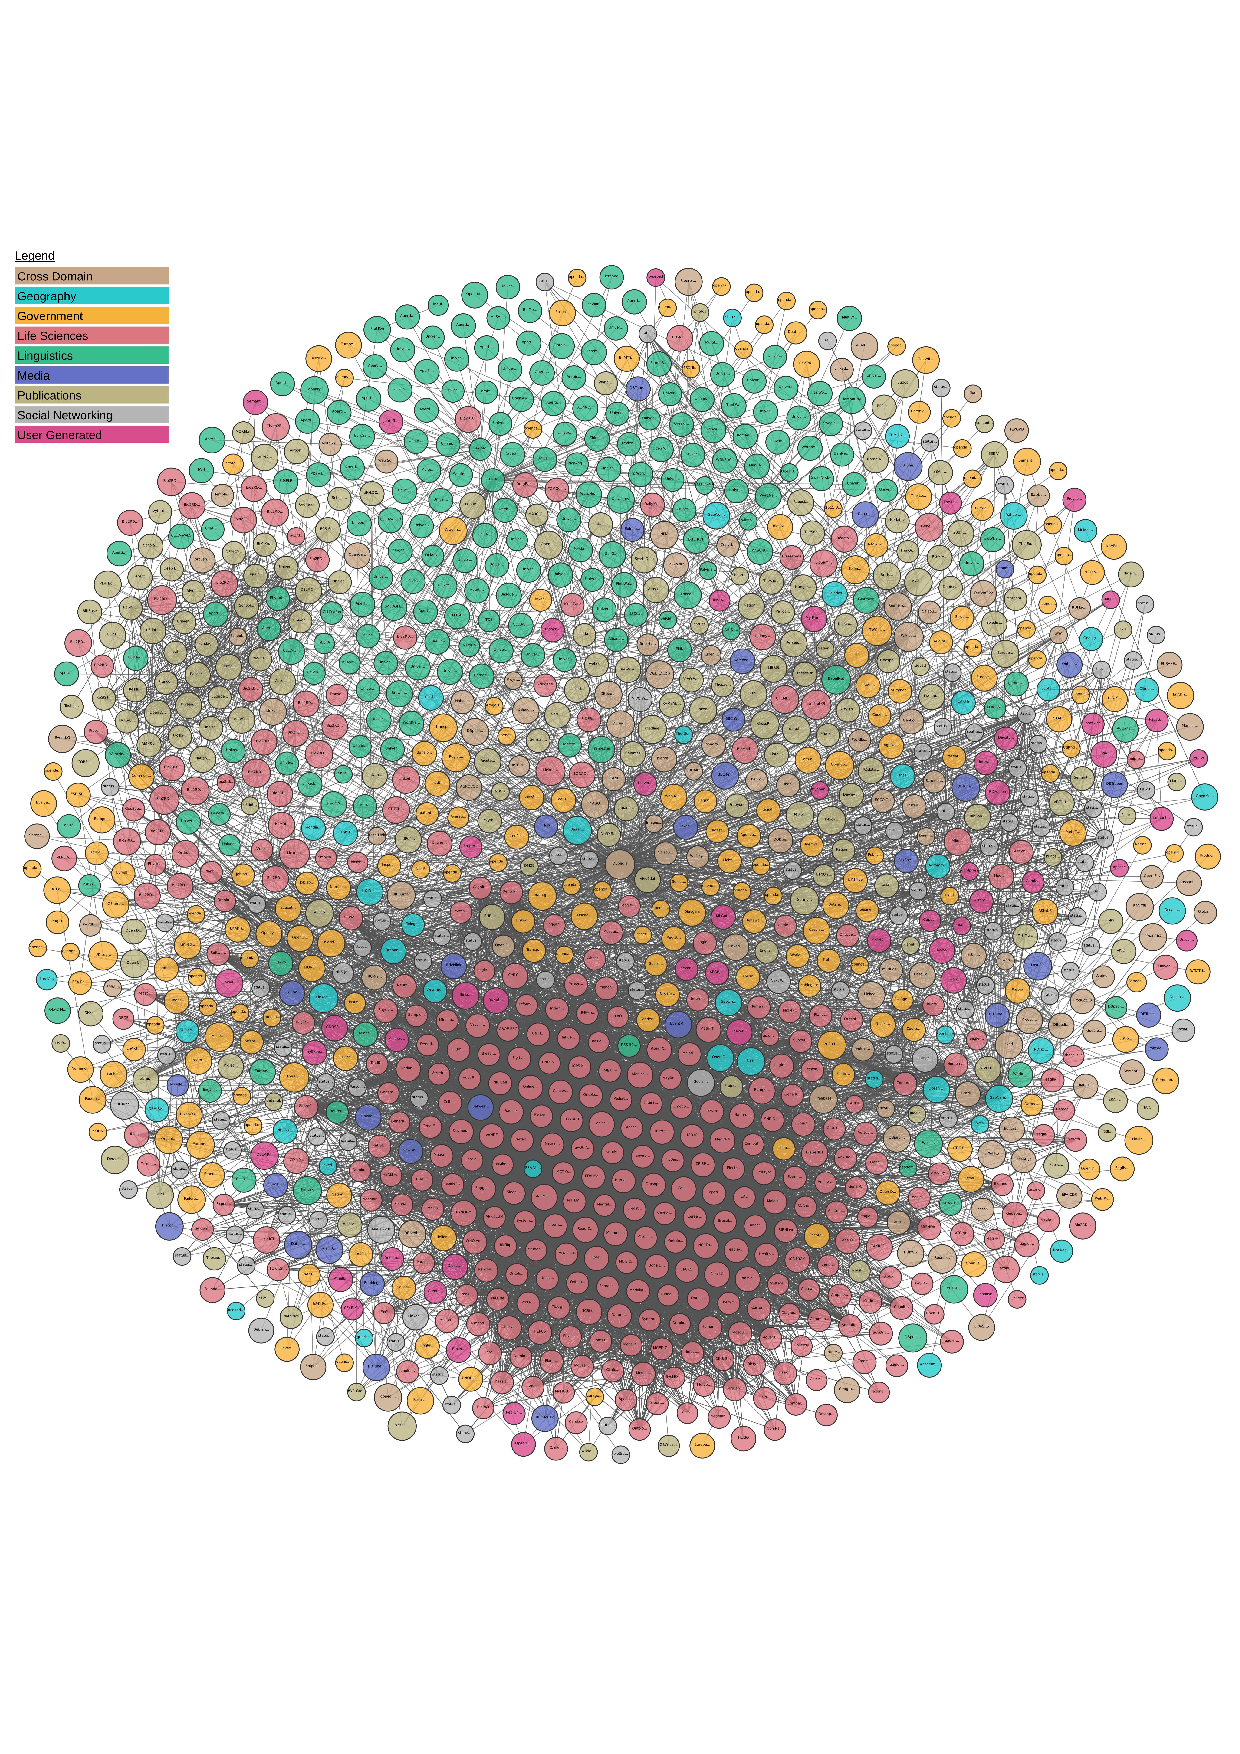
\includegraphics[width=11cm]{./figures/part1/lod-cloud.pdf}
    \caption{关联数据}
   \label{fig:linkeddata}
\end{center}
\end{figure}


\subsection{常见中文知识图谱数据集}\label{sec:ChineseDatasets}
\textbf{PKUBase.}
PKUBase

\textbf{CN-DBpedia.}
CN-DBpedia\cite{DBLP:CNDBpedia} CN-DBpedia是由复旦大学知识工场实验室研发并维护的大规模通用领域结构化百科知识图谱数据集。CN-DBpedia前身是复旦大学GDM中文知识图谱,是国内最早推出的也是目前最大规模的开放百科中文知识图谱数据集。CN-DBpedia涵盖数千万实体和数亿级的关系,相关知识服务API累计调用量已达6亿次。
CN-DBpedia以通用的百科知识沉淀为主线,以垂直纵深领域图谱积累为支线,致力于为机器语义理解提供了丰富的背景知识,为实现机器语言认知提供必要支撑。

CN-DBpedia已经从百科领域延伸至法律、工商、金融、文娱、科技、军事、教育、医疗等十多个垂直领域,为各类行业智能化应用提供支撑性知识服务,目前已有近百家单位在使用。
CN-DBpedia具有体量巨大、质量精良、实时更新、丰富的API服务等特色。CN-DBpedia已经成为业界开放中文知识图谱的首选。基于CN-DBpedia的知识图谱构建与应用能力已经输出并应用在华为、小I机器人、中国电信、中国移动、同花顺等业界领军企业的产品与解决方案中。

CN-DBpedia提供全套API,并且免费开放使用。详细下载地址,可见http://kw.fudan.edu.cn/cndbpedia/intro/。



\subsection{常见外文知识图谱数据集}\label{sec:EnglishDatasets}
\textbf{DBpedia.}
DBpedia\cite{DBLP:DBpedia}
2007年开放。
目标是构建一个社区,通过社区成员定义和撰写准确的抽取模板,进而从维基百科中抽取结构信息,并将其发布到Web上。
社区通过人工的方式构建分类:
280个类别
覆盖约50%的维基百科实体


\textbf{YAGO.}
YAGO\cite{DBLP:YAGO,DBLP:YAGO2,DBLP:YAGO3}

\textbf{Freebase.}
Freebase\cite{url:Freebase}
2007年Metaweb公司发布。
2010年被Google收购。
大规模协同构建知识库。
从Wikipedia和其他数据源(如 IMDB、MusicBrainz)中导入知识
核心思想:
在Wikipedia中,人们编辑文章
在Freebase中,人们编辑结构化知识



\chapter{知识图谱的查询语言---SPARQL}\label{sec:SPARQLIntroduction}
\section{SPARQL简介}
SPARQL是W3C制定的RDF图数据的标准查询语言。SPARQL从语法上借鉴了SQL,同样属于声明式查询语言。SPARQL 1.1是一组规范,提供用于在Web或RDF存储中查询和操作RDF图形内容的语言和协议。最新的SPARQL 1.1版本为有效查询RDF 图而专门设计了三元组模式、子图模式、属性路径等多种查询机制。几乎全部的RDF三元组数据库都实现了 SPARQL语言。SPARQL 提供了强大的基于图形匹配的查询功能,里面的主要功能有:提炼查询结果(ORDER BY, PROJECTION,DISTINCT, REDUCED, OFFSET, LIMIT)、可选匹配 (optional)、值约束条件(filter)、替换匹配、以及直接回答 YES/NO 等其他形式的查询。最简单的图形模式是三元组。

从SPARQL的全称我们可以知道,其由两个部分组成:协议和查询语言。


\begin{enumerate}
  \item 查询语言很好理解,就像SQL用于查询关系数据库中的数据,XQuery用于查询XML数据,SPARQL用于查询RDF数据。
  \item 协议是指我们可以通过HTTP协议在客户端和SPARQL服务器(SPARQL endpoint)之间传输查询和结果,这也是和其他查询语言最大的区别。
\end{enumerate}


\subsection{IRI}
SPARQL语言包括IRI,它是省略空格的RDF URI引用的子集。请注意,SPARQL查询中的所有IRI都是绝对的; 它们可能包含也可能不包含片段标识符。IRI包括URI和URL。解析SPARQL语法中的缩写形式(相对IRI和前缀名称)以生成绝对IRI。在SPARQL语言中包括IRIs,它可以用来代替RDF中URIs这样的命名空间。在SPARQL查询中所有的IRIs是绝对的,它们有时包括有时不包括标识符。IRIs包括URIs和URLs。其中表示带前缀的名字,分隔符“<”和“>”不是IRIs的组成部分。



PREFIX关键字是把前缀标签和IRI(Internationalized Resource Identifiers)连接起来,一个有前缀的名称是由一个带前缀的标签和一个本地的名称所组成中,其中由冒号“:”来分开。这个有前缀的名称可以通过连接IRI的前缀和本地部分来映射到该nu上,这个前缀或本地名称可能是空的。值得注意的是SPARQL的本地名称开头可以是数字,而XML的本地名称则不可。SPARQL本地名称也允许有非字母或数字的符号(如反斜杠ns:id\=123)存在于 IRIs 中。


常用的命名空间前缀与IRI的关系如表\ref{table:PrefixMapping}所示。

\begin{table}\label{table:PrefixMapping}
\caption{常用的命名空间前缀与IRI对应表}
\begin{tabular}{ll}
  \hline
  % after \\: \hline or \cline{col1-col2} \cline{col3-col4} ...
  \textbf{字首} &\textbf{IRI}\\
  \hline
 rdfs: & http://www.w3.org/2000/01/rdf-schema\# \\
  rdf: & http://www.w3.org/1999/02/22-rdf-syntax-ns\# \\
 xsd: & http://www.w3.org/2001/XMLSchema\# \\
  fn: & http://www.w3.org/2005/xpath-functions\# \\
 sfn: & http://www.w3.org/ns/sparql\# \\
  \hline
\end{tabular}
\end{table}

\subsection{SPARQL语法中的文字表示}
SPARQL在使用上与其他的语言一样,有自己的语言规范。SPARQL语法共有5部分构成:命名空间(NS)、数据集(RDF Dataset)、查询方式(QF)、图模式(GP)、结果修饰(SM),表\ref{table:QueryParts}显示了以上5部分查询语句的示例。


\begin{table}\label{table:QueryParts}
\caption{查询语句各部分示例}
\begin{tabular}{ll}
  \hline
  % after \\: \hline or \cline{col1-col2} \cline{col3-col4} ...
  \textbf{组成部分} &\textbf{示例}\\
  \hline
 NS & prefix foaf: <http://xmlns.com/foaf/0.1/> \\
  RDF Dataset & FROM NAMED  <http://example.org/foaf/bobFoaf> \\
 QF & SELECT ?name ?mbox \\
  GP & WHERE  { { ?book dc10:title ?title .  ?book dc10:creator ?author }
UNION
{ ?book dc11:title ?title .  ?book dc11:creator ?author }
}
 \\
 SM & ORDER BY ?X \\
  \hline
\end{tabular}
\end{table}


语法中的文字(Literals)是包含在双引号或单引号中的字符串(String),它通常伴有一个可选的语义标签(通过@表示),或是一个可选的RI数据类型(通过AA表示)或者一个带前缀的名字。为了方便起见,整数在一般情况下可以接书写而不用附加的数值类型,在运用的时候会被自动解释为xsd:integer这个数据类型。在数字中有小数点而没有指数的十进制数被理解为xsd:decimal类型的文字,如果是带指数的数字会被解释为xsd:double类型,另外,xsd:boolean类型的数值可以直接写为true或false[47]。在文字中包含换行符或者引号或者描述过长的情况下,SPARQL语法允许使用两个或三个单引号来对其描述。表3是对SPARQL语法中的文字的使用的描述。

\section{SPARQL操作符}

\section{SPARQL 1.1上的高级运算符}


\part{知识图谱构建}
%\chapter{֪ʶͼ�׹���}\label{sec:construction}
\section{֪ʶ��ʾ}

\section{���ڽṹ�����ݵ�֪ʶͼ�׹���}

\section{���ڰ�ṹ�����ݵ�֪ʶͼ�׹���}

\section{���ڷǽṹ�����ݵ�֪ʶͼ�׹���}
%\chapter{��������}\label{sec:quality}



\part{知识图谱管理}
\input{./body/part2/rdf-management}
\chapter{基于关系数据库技术的知识图谱管理系统}\label{sec:RelationSystem}

\begin{figure}[h]
\begin{center}
   \includegraphics[width=11cm]{./figures/part2/rdf3x-index.pdf}
    \caption{全索引结构}
   \label{fig:rdf3xindex}
\end{center}
\end{figure}

\begin{figure}[h]
\begin{center}
   \includegraphics[width=11cm]{./figures/part2/selection.pdf}
    \caption{选择}
   \label{fig:selection}
\end{center}
\end{figure}

\begin{figure}[h]
\begin{center}
   \includegraphics[width=11cm]{./figures/part2/projection.pdf}
    \caption{选择}
   \label{fig:selection}
\end{center}
\end{figure}

\begin{figure}[h]
\begin{center}
   \includegraphics[width=11cm]{./figures/part2/join.pdf}
    \caption{连接}
   \label{fig:join}
\end{center}
\end{figure}
\chapter{基于图数据库技术的知识图谱管理系统}\label{sec:GraphSystem}

%\input{./body/part2/gStore-advanced}

%\part{分布式版知识图谱管理系统}
%\input{./body/part3/cloud-system}
%\chapter{特制的分布式知识图谱管理系统}\label{sec:SpecializedSystem}
%\input{./body/part3/gStoreD}

\part{应用案例}
\chapter{图数据库系统gStore使用基础}\label{sec:gStore}
\chapter{金融知识图谱应用案例}\label{sec:finance}
\input{./body/part3/medicine}
\input{./body/part3/robot}



\printbibliography

\end{document}

